\documentclass[12pt]{scrartcl}

\usepackage[utf8]{inputenc}
\usepackage[IL2]{fontenc}
\usepackage[czech]{babel}
\usepackage{graphicx}
\usepackage{hyperref}
\usepackage{amsmath}
\usepackage[]{algorithm2e}
\usepackage{enumitem}
\usepackage{gensymb}

\subject{Západočeská univerzita v\nobreakspace Plzni\\Fakulta aplikovaných věd\\KIV/KPG}
\author{Pavel Zelenka\\A16B0176P\\zelenkap@students.zcu.cz}
\date{\today}
\title{Fraktály}

\begin{document}
\maketitle
\pagenumbering{gobble}
\newpage
\pagenumbering{arabic}
\newpage
\section{Zadání}
	
\paragraph{}
Zadáním úkolu je vytvoření nového programu nebo rozšíření programu ze cvičení, tak aby vykresloval fraktály, které nebyly na cvičení.

\section{Analýza problému}

\paragraph{}
\textbf{Fraktál} je\nobreakspace seběpodobný útvar, to znamená, že lze pozorovat stále opakující\nobreakspace se tvar. Mezi známe fraktály patří Sierpińského koberec, Sierpińského trojúhelník, či křivka vyplňující prostor.

V této práci se budu zabývat křivka vyplňující prostor, konkrétně \textbf{Hilbertovou křivkou}.

\section{Popis řešení}

\paragraph{}
Vykreslování probíhá ve\nobreakspace třídě \emph{Drawing}. Algortitmy fraktálů\nobreakspace se nacházejí v balíčku \emph{fractal}.

\subsection{Hilbertova křivka}
\paragraph{}
V práci je implementován algoritmus, který index bodu Hilbertovy křivky převádí do kartézské soustavy souřadnic bez použití rekurze. Algoritmus předpokládá, že bod s indexem $0$ je na pozici $[0,0]$. V první iteraci existují právě 4 body a počáteční křivka je pevně daná.

\paragraph{}
Pozice následujících bodů se dopočítávají podle indexu. Poslední 2 bity označují umístění bodu v rámci čtveřice bodů (tj.\nobreakspace tvar křivky v první iteraci), následující dvojice bitů označuje umístění předešlé čtveřice bodů v rámci šestnáctice bodů (tj.\nobreakspace křivka v druhé iteraci).

\begin{figure}[!ht]
	\centering
	\label{obr:polekolizi}
	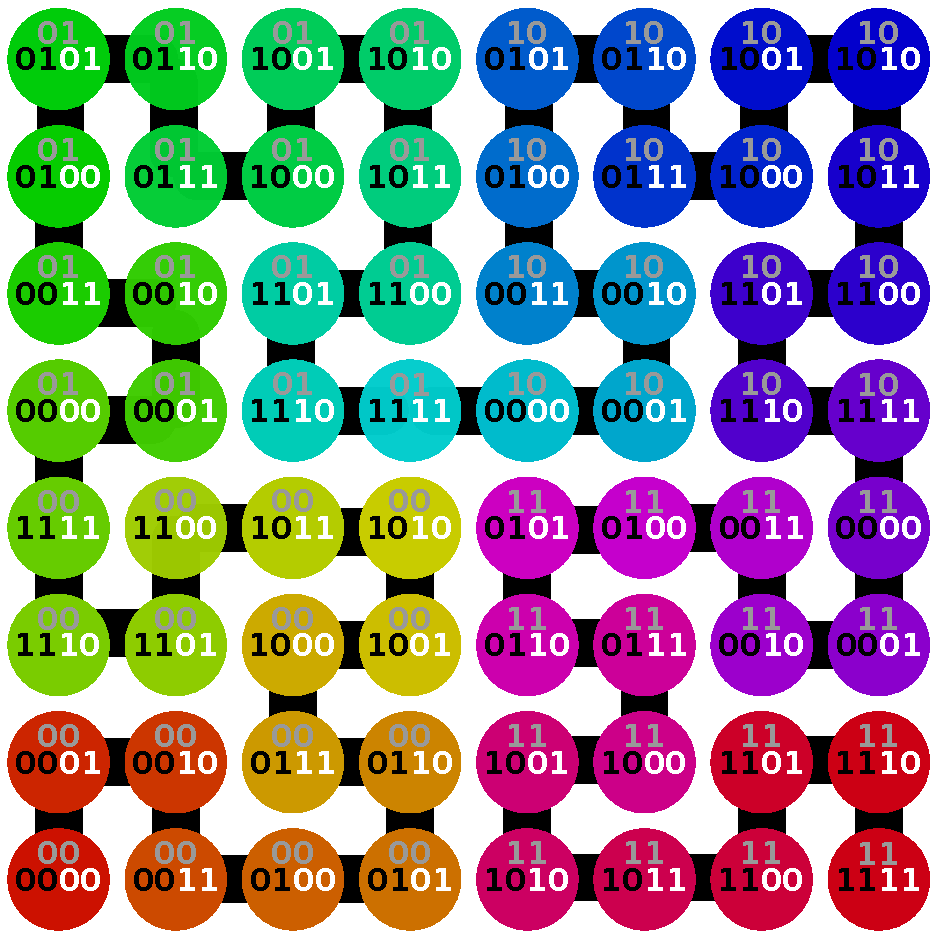
\includegraphics[width=0.85\textwidth,natwidth=1,natheight=1]{hilbert.pdf}
	\caption{Indexy bodů v třetí iteraci}
\end{figure}

\newpage
\section{Uživatelská dokumentace}

\paragraph{}
Spuštění aplikace se\nobreakspace provede souborem \texttt{Fractal.jar}, který se nachází ve složce \emph{App}.

\begin{figure}[!ht]
	\centering
	\label{obr:polekolizi}
	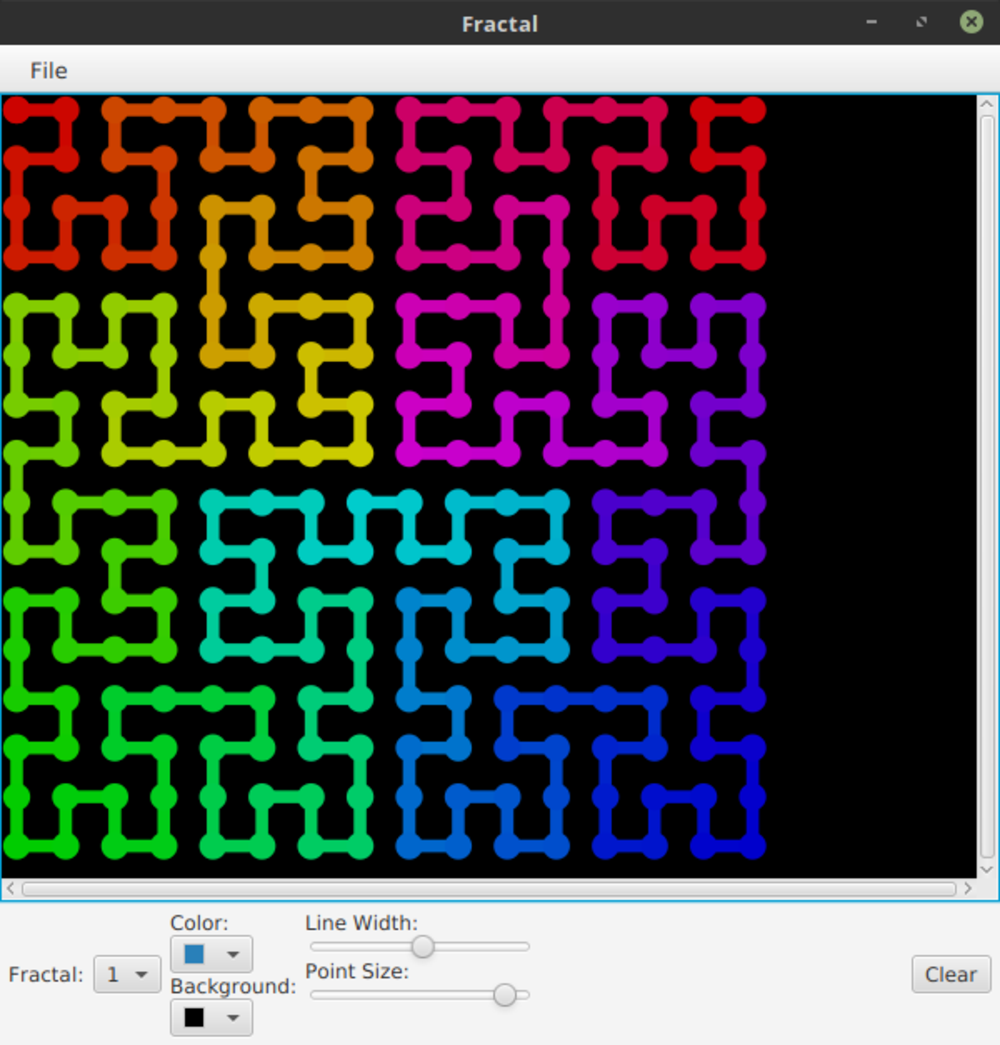
\includegraphics[width=0.85\textwidth,natwidth=1,natheight=1]{app_gui.pdf}
	\caption{Okno aplikace}
\end{figure}

\newpage
\section{Závěr}
\paragraph{}
Úkol jsem řešil v\nobreakspace jazyce \texttt{Java} s použitím grafických knihoven \texttt{JavaFX}. V knihovně JavaFX mi nevyhovovala implementace \texttt{Point2D}, kde není možná změna pozice existujícího bodu, proto je v odevdávané aplikaci vlastní implementace bodu. Nepodařilo\nobreakspace se\nobreakspace mi zjistit, zdali existuje řešení bez nutnosti vlastní implementace.

\section{Reference}

\end{document}
